\subsection{The ANTLR Workflow}
\label{subsec:antlr_workflow}

In this work we will be using a modified version of ANTLR's default C grammar file. The details of the modifications will be covered later in this section. The tools generated by ANTLR included a lexer, parser, and listener. A lexer is a tool that takes an input string and converts it to a set of tokens in accordance with the rules set out by the grammar file. A parser then takes these tokens and returns a parse tree, also based on the grammar's rules. A parse tree is a tree graph structure that represents the syntactical structure of the parsed file. The leaf nodes are the characters that are directly in the file with the parent nodes defining the semantic context its children fall into. Figure \ref{fig:hello_world} shows an example parse tree for a "Hello world" function using the C grammar. From the parse tree, a breadth-first search can be conducted. The listener instantiates events every time a node in the tree is entered or exited where nothing happens. The user can then customize these events to execute an arbitrary block of code with a context provided as to the location in the tree.

\begin{figure}[ht]
    \centering
    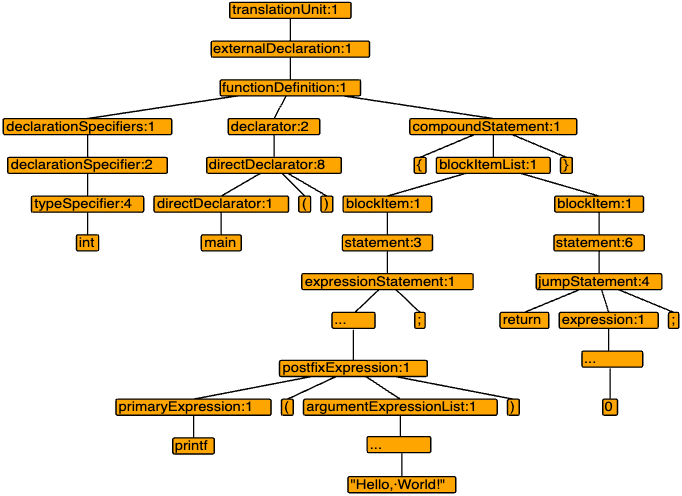
\includegraphics[width=1.0\linewidth]{figures/antlr_hello_world.png} \\
    \caption{An ANTLR parse tree for hello world in C. Note that vertical chains of nested contexts are replaced with "..." for brevity.}
    \label{fig:hello_world}
\end{figure}

In the hello world example in Figure \ref{fig:hello_world}, a user defined block of code could be run every time a directDeclarator context is entered to capture its name if the name exists and the directDeclarator is the grandchild of a functionDefinition. This would result in the name of the function, main, being captured. These types of listener events were defined in the custom listener for this work in order to capture the dependency information for the definitions and instantiations of the types of interest outlined in Section \ref{subsec:graph_construction}. Macros and include statements were covered with regex rather than with the listener as ANTLR's C grammar file doesn't capture pre-processor directives, pre-processor directives are non-semantic in nature as they always are the string which directly follows their directive (\#include and \#define respectively), and it is simpler to use RegEx than to create definitions for them in the grammar files.

As previously noted, the C grammar file provided by ANTLR required modifications in order to be useful for this project. The primary concern was the lack of a definition for macros which, as discussed in Section \ref{sec:intro} and demonstrated in Table \ref{tab:library_metadata} of Section \ref{subsec:workloads}, are a significant component in HPC code-bases. This was a significant undertaking as macros can appear very similar and/or very dis-similar to functions definitions and instantiations. The complexity from this came from making the macro grammar components general enough to cover a plethora of edge cases while also specific enough as to interpret non-macros as macros. Macros can also take in anything as an argument which created more complexities as anything was inclusive of more exotic components such as operators, reserved identifiers, other macros, and function instantiations and declarations. The final grammar file used was not able to remove 100\% of the errors that were encountered, but none of the errors lead to termination conditions and the number of errors in proportion to the size of the code-bases were insignificant as will be explored in Section \ref{subsec:workloads}.

